\documentclass[11pt]{article}
\usepackage[pdftex]{graphicx}

\usepackage{henrian-basic}
\usepackage{henrian-homework}
\usepackage{chngpage}

\usepackage{amsmath}
\usepackage{float}
\usepackage{natbib}
\bibliographystyle{plainnat}
\bibpunct{(}{)}{,}{a}{,}{,}

\makeHeaders{Machine Learning: Homework 8}

\begin{document}

\begin{itemize}
  \item \textbf{Email}: chrisbrown@utexas.edu
  \item \textbf{EID}: chb595
\end{itemize}

\section{Genetic Algorithms}

\subsection{My algorithm}

I used a pool of 200 solvers (every generation had a population of 200), with a pretty large carryover (k) rate: 150. I was finding small population over many generation was more efficient than large population over few generations, and that I was losing a lot of diversity if my carryover rate was small. In a Genetic Algorithm (GA) scenario that required a broader search space, the opposite would probably be better: to have a greater number of solvers, less carryover, and fewer iterations. The sorting problem for this homework is quite narrow, though, which means that it has a narrower search than other problems might have.

I used a pool of 20 parasites, which evolved in much the same way as the solvers, but without crossover; I only used biased selection, based on difficulty, and a higher mutation rate than that experienced by the solvers.

In brief, my algorithm proceeds as detailed in the following enumeration:
\begin{enumerate}[1.]
  \item I generated 200 solutions and 20 parasites, by random. Each solution started out with 10 to 50 ``swaps'' (pairs of integers, where each integer is in the range [0, 15]). The parasites were simply lists of 16 integers, all in the range [10 and 100), to make results and debugging easier. They could be any number, and the algorithm would work the same way.
  \item I tried out all the solvers on all the parasites once per generation, and ranked the best solvers based on how many mistakes they made, total. I had trouble factoring solver length (number of swaps) into the fitness function, so I curtailed solver length by a biased crossover process, which I will explain later. I also ranked the parasites based on the number of mistakes made on them by all the solvers.
  \item I selected the top solvers proportional to the number of mistakes made by the worst, \emph{times two}, minus the number of mistakes made by each solver. If I did not bias the remapping this way, the worst solvers would have fitness scores of 0, and thus absolutely no chance of being selected for survival.

  The probability of picking some solver $s$, then, was:
  \[
    p(s) = \frac{(2 \cdot \stackrel{max}{r} mistakes(r)) - mistakes(s)}{\sum_t (2 \cdot \stackrel{max}{r} mistakes(r)) -mistakes(t)}
  \]

  Note that the fitness plot in \S\ref{sec:results} depicts absolute number of mistakes. This remapping was simply done to make picking the top solvers more efficient.

  According to this weighting, I selected 50 pairs of solvers, and merged+split each with crossover, producing 100 new solvers. I selected another 100 solvers simply by weighted random, using the $p(s)$ measure.

  For each of the 200 solvers, with probability 0.1, I exchanged one of their swaps with a random new swap. Thus, on average, 20 solvers would have gotten one of their swaps randomly replaced each generation.

  The next generation of parasites was chosen in much the same way; the best are selected according to the mistakes they accrued from the solvers (mistakes are good things, for parasites), and then each parasite undergoes a mutation of exactly one of their entries.
  \item If any of the solvers can solve all the parasites in the pool without making any mistakes, we are finished. Otherwise, return to step 2, and proceed from there.
\end{enumerate}

\subsection{The fitness function}

While I described how I used the number of mistakes, I did not describe how I counted them. I tried two different methods. After using a solver to sort a parasite (which was a simple matter of iterating through the pairs of swaps, and swapping two entries in the parasite if the entry pointed to by the left side of the swap was greater than the entry pointed to by the right side of the swap):
\begin{enumerate}[a.]
  \item Compare each pair of items in the sorted result, to see if they are correctly sorted (less than or equal). This required 120 (= 16 choose 2) comparisons.
  \item Compare each adjacent pair of items to see if they are correctly sorted (less than or equal). This required 15 (= 16 - 1) comparisons.
\end{enumerate}
I found the (a) was the only viable option; it converged much more quickly than (b). In fact, (b) did not converge during the time I allowed the algorithm to run.

I think this is due to the incremental gains provided by the (a) method. Since I was only evaluating against a small set of parasites, I only got a small selection of feedback for any set of swaps. For example, if I sorted a sequence like [5, 99, 1] as [1, 99, 5], method (b) would find this to be no improvement over the original sequence. However, method (a) would more accurately reflect that this result is more sorted than the original, just not completely sorted.


\subsection{Crossover}
The intuition behind crossover is that if you take two strings from two good, but not perfect, candidates, you might happen to factor out the bad parts, and keep the good parts. It's really just a kind of guided mutation, because as with any mutation, you're going to produce many more outright failures and abominations, but certainly fewer than if we simply produced random mutations, or random new individuals.

I tried various versions of crossover; for two strings A and B:
\begin{enumerate}[a.]
  \item One cut:
    \[
      \frac{abcd\mathbf{ef}}{zyxw\mathbf{vu}} \to \frac{abcd\mathbf{vu}}{zyxw\mathbf{ef}}
    \]
  \item Two cuts:
    \[
      \frac{ab\mathbf{cd}ef}{zy\mathbf{xw}vu} \to \frac{ab\mathbf{xw}ef}{zy\mathbf{cd}vu}
    \]
  \item Two cuts per string:
    \[
      \frac{ab\mathbf{cde}f}{zy\mathbf{x}wvu} \to \frac{ab\mathbf{x}ef}{zy\mathbf{cde}wvu}
    \]
\end{enumerate}
I did not formally compare the different approaches, but the last seemed to work the best. (a) and (b) are basically the same; picture the sequence of pairs of indices as a ring, and it becomes clear that (a) is just (b) while setting the second cut to the end of the string, as noted by \citet{whitley:1993}, who credits this observation to \citet{dejong:1975}.

The alternative, (c), is even more flexible than (b), by which I mean that it will generate more variety. A string of one swap could become a string of two in one crossover. While this is unnatural when considered in the context of biological crossover, it seems more suitable here because it is a generalization of (b), and we want to try out as many different combinations as possible, as quickly as possible. The human genome is not functionally homogeneous; the first percent and the last percent most likely correspond to very different operations. But each swap in the sequence we consider in this problem is the same operation. Certainly, the order of swaps matters, but not as much as in a complex biological genome.

Because I was not able to figure out a good way to weight the cost of lengthy swap sequences against mistakes made on each parasite, I used the crossover mechanism to curb the length of the strings. When selecting the number of swaps to pull from each solver, I used a draw from the truncated Normal distribution instead of the uniform, in order to bias the length lower. The truncation was simple; I just took the absolute value of a $\mathcal{N}(0, \frac{#swaps}{10})$, to determine how much of the string to swap out to the other side of the crossover. This is not as principled as incorporating the number of swaps into the fitness function would have been, but it was more successful in my implementation. I did not use the optimization of de-duplicating pairs of identical swaps to reduce the total number, since that seemed arbitrary and ad-hoc---more of a programmatic hack than algorithmic optimization. However, checking the final result provided at the end of this write-up, that optimization would have only reduced the total number of swaps by three.

The length of the string was also naturally minimized, in some small way, by the fact that any swap of (a, b), where a > b, would likely hurt the end result. Thus, swaps like those were naturally selected out of the solution by the standard mistake-counting fitness function.

\subsection{Mutation}
Mutation is simpler than crossover; in my implementation, there is one parameter that determines the probability that we will mutate a given candidate in a particular generation. I take the simplest route; with a constant probability $p_{mutation}$, I replace one swap in a candidate, chosen by random, with a completely random new swap. There are variations; we could also specify how many mutations to execute, but the same effect is achieved over several generations by simply choosing a different $p_{mutation}$. Or we could mutate a swap by only changing only one of the indices, or by changing the indices by only a small amount. However, I only implemented the simplest approach, where I fully replace one swap with an entirely random new pair of indices.

\section{Results}
\label{sec:results}

In Figure \ref{fig:best-solution-performance}, you can see the best solution's performance, plotted as the number of generations progresses. As you can see, it converges pretty quickly---it took just over 600 generations.

\begin{figure}[H]
  \centering
  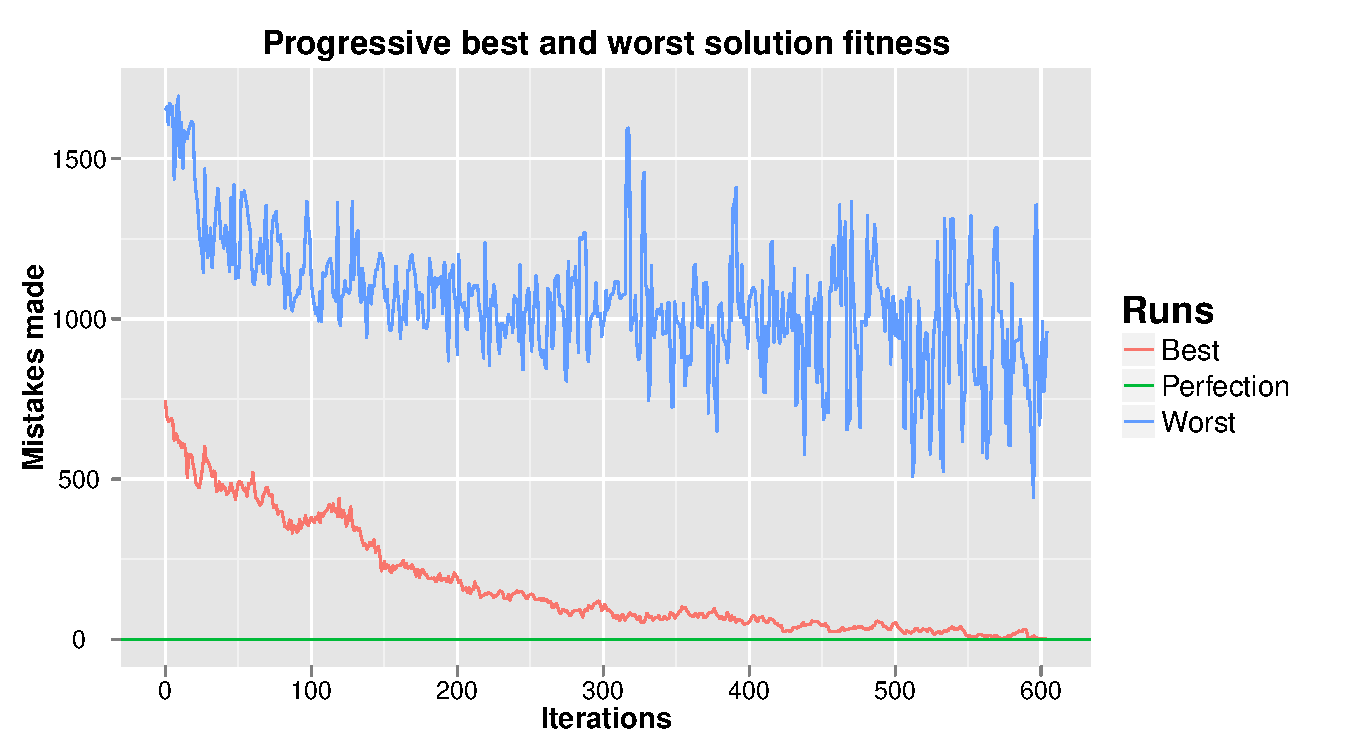
\includegraphics[width=0.95\textwidth]{results/output-i600-fitness.pdf}
  \caption{The best solution's performance, over generation. Lower is better, because my fitness function measured mistakes made in ordering.}
  \label{fig:best-solution-performance}
\end{figure}

\noindent
And in Figure \ref{fig:best-solution-length}, I show see the length of the best solution, plotted against the number of generations elapsed.

\begin{figure}[H]
  \centering
  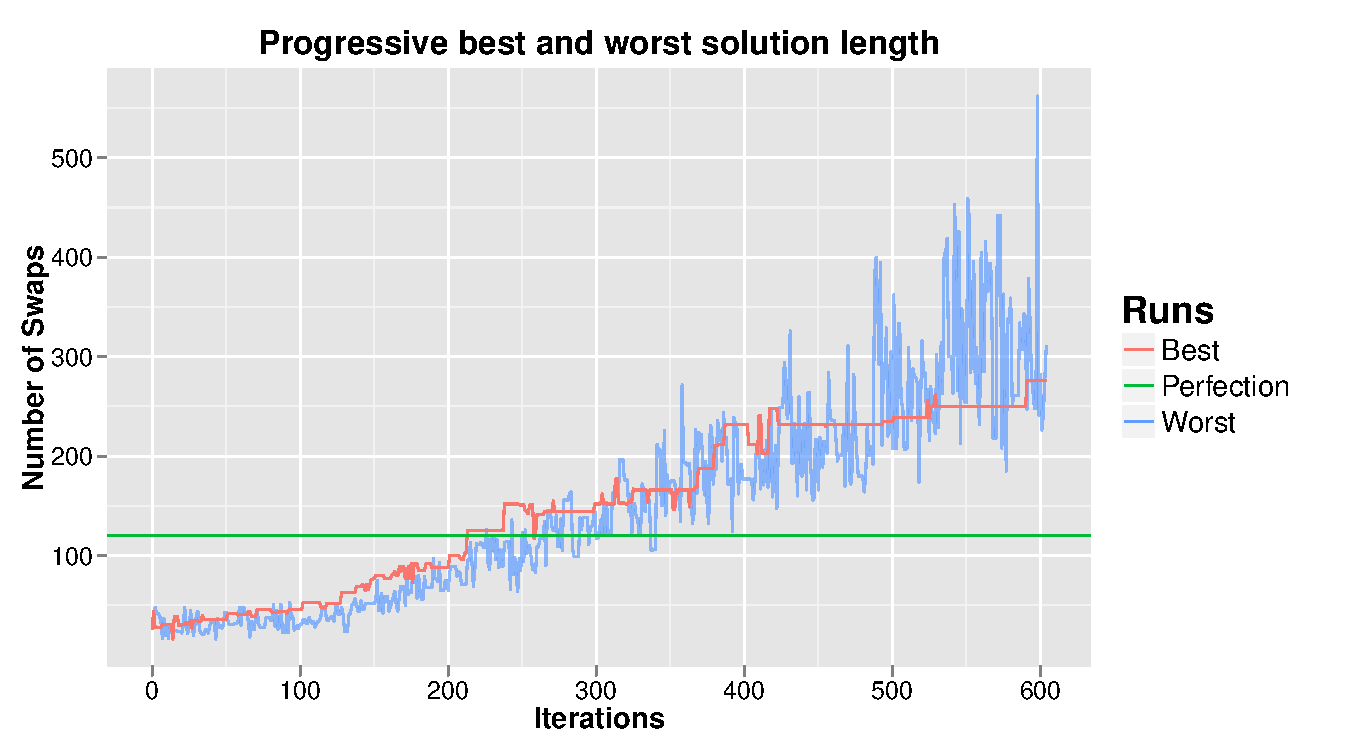
\includegraphics[width=0.95\textwidth]{results/output-i600-length.pdf}
  \caption{The best solution's length, over generation.}
  \label{fig:best-solution-length}
\end{figure}

\subsection{Solution}

Here is a final solution, a final parasite sequence, and the solution's sort of that sequence:

\begin{figure}[H]
  \begin{adjustwidth}{.5in}{.5in}
    \begin{footnotesize}
      (2,13) (2,2) (7,3) (8,4) (4,2) (7,14) (9,10) (12,7) (2,2) (11,2) (9,14) (4,12) (13,2) (7,4) (5,9) (2,2) (5,5) (4,2) (7,14) (8,7) (9,11) (15,5) (12,12) (11,13) (10,11) (10,7) (12,7) (1,9) (9,10) (7,4) (9,11) (15,5) (12,12) (12,7) (5,9) (4,12) (6,5) (2,9) (7,8) (7,3) (10,14) (7,14) (7,8) (4,12) (9,10) (2,15) (8,0) (3,14) (1,12) (8,6) (12,7) (6,15) (5,9) (15,2) (2,9) (4,12) (9,10) (2,15) (8,0) (3,14) (1,12) (8,6) (12,7) (6,15) (12,7) (1,7) (14,11) (9,10) (15,11) (6,7) (10,7) (7,3) (11,3) (15,5) (2,2) (7,14) (9,10) (15,2) (10,11) (11,3) (7,8) (15,12) (9,3) (2,9) (6,9) (6,7) (15,12) (9,3) (12,7) (2,9) (10,11) (7,8) (7,8) (7,4) (5,9) (12,12) (2,15) (8,0) (7,4) (5,9) (2,2) (7,3) (8,4) (4,2) (7,14) (9,10) (12,7) (2,2) (5,5) (9,14) (4,12) (10,14) (7,14) (7,8) (4,12) (9,10) (2,15) (8,0) (3,14) (1,12) (8,6) (5,9) (15,2) (6,7) (12,7) (12,7) (6,15) (6,15) (5,9) (1,12) (8,6) (12,7) (6,15) (5,9) (15,2) (14,0) (13,2) (7,4) (5,9) (2,2) (5,5) (6,7) (10,7) (7,3) (9,10) (12,12) (15,2) (9,10) (2,9) (10,11) (7,8) (15,12) (9,3) (12,7) (15,2) (9,10) (11,5) (10,11) (7,8) (15,12) (11,3) (12,7) (5,9) (2,2) (6,9) (7,8) (11,13) (10,11) (9,11) (3,14) (1,12) (8,6) (13,0) (6,15) (5,9) (15,2) (14,0) (13,2) (7,4) (5,9) (2,2) (5,5) (4,2) (7,14) (8,7) (9,11) (15,5) (12,12) (11,13) (10,11) (10,7) (12,7) (1,9) (9,10) (7,4) (9,11) (15,5) (12,12) (12,7) (5,9) (4,12) (6,5) (2,9) (7,8) (7,3) (10,14) (7,14) (7,8) (4,12) (9,10) (2,15) (8,0) (3,14) (1,12) (8,6) (12,7) (6,15) (5,9) (15,2) (14,0) (13,2) (7,4) (5,9) (2,2) (5,5) (4,2) (7,14) (8,7) (9,11) (15,5) (12,12) (11,13) (10,11) (10,7) (12,7) (1,7) (15,11) (6,7) (10,7) (7,3) (11,3) (15,5) (2,2) (12,12) (2,13) (7,8) (15,12) (11,13) (10,11) (10,7) (7,3) (4,12) (12,12) (15,2) (9,10) (2,9) (10,11) (9,10) (1,2) (2,13) (12,12) (15,2) (9,10) (2,9) (10,11) (7,8) (15,12) (9,3) (12,7) (9,11) (0,15) (0,0) (13,14) (1,15) (3,12) (8,10)
    \end{footnotesize}
  \end{adjustwidth}
  \caption{The final solution. Total length: 276.}
\end{figure}

\noindent
276 is a lot more than the perfect solution, which is 120, and a smarter fitness function and broader parasite pool could probably bring the number down. However, as I mentioned above, it was difficult to know how to weight the penalty for longer swap sequences.

\begin{figure}[H]
  \begin{small}
    \begin{center}
      \begin{tabular}{rcccccccccccccccc}
        % ' & '.join(s.split(', '))
        Parasite: & 59 & 80 & 81 & 41 & 88 & 83 & 56 & 76 & 92 & 62 & 19 & 98 & 98 & 69 & 91 & 55 \\
        Solution: & 19 & 41 & 55 & 56 & 59 & 62 & 69 & 76 & 80 & 81 & 83 & 88 & 91 & 92 & 98 & 98 \\
      \end{tabular}
    \end{center}
  \end{small}
  \caption{A sort by the final solution of one of the most difficult parasites.}
\end{figure}

\bibliography{/Volumes/Zooey/Dropbox/ut/tex/liography}

\end{document}

% The final homework is posted and due Tuesday April 24 at 11:59pm. You may use Python or Java if you prefer.

a = [5, 10, 9] (gt, lt)
b = [5, 10, 4] (gt, lt)

perfect_swaps = [(0, 1), (0, 2), (1, 2)]
a_sufficient_swaps = [(1, 2)]
a_sufficient_swaps = [(0, 2), (1, 2)] or [(1, 2), (0, 1)]

